\section{Training}

The library is implemented in C++ and provides essential components for constructing and training neural networks, such as layers, loss functions, and training utilities. In this section, we explain how to build a model, data flow, and training pipeline using our library.

\subsection{Model Construction with \texttt{Sequential}}

The model is defined using the \texttt{Sequential} class from the \texttt{cnn\_library}, which provides a linear stack of layers. Each layer conforms to a standard interface, making it easy to chain different types of operations.

The model is created in the \texttt{create\_mnist\_model()} function, which takes the input size, batch size, and number of output classes as parameters. The architecture consists of several fully connected (\texttt{Linear}) layers, interleaved with \texttt{ReLU} activation layers, and concludes with a \texttt{Softmax} output layer. The structure of the model is as follows:

\begin{itemize}
    \item Linear Layer: $784 \rightarrow 1024$
    \item ReLU Activation
    \item Linear Layer: $1024 \rightarrow 1024$
    \item ReLU Activation
    \item Linear Layer: $1024 \rightarrow 512$
    \item ReLU Activation
    \item Linear Layer: $512 \rightarrow 512$
    \item ReLU Activation
    \item Linear Layer: $512 \rightarrow 10$
    \item Softmax Layer (for classification)
\end{itemize}

The model is built by calling \texttt{addLayer()} repeatedly on a \texttt{Sequential} object, allowing layers to be appended in a modular fashion.

\subsection{Loss Function and Device Configuration}

We use \texttt{Cross\_Entropy\_Loss}, which is suitable for multi-class classification problems like MNIST. The loss function calculates the difference between the predicted probability distribution and the true label distribution.

The model and the loss function both support device configuration. By calling \texttt{setDevice(1)}, we assign GPU execution to accelerate training. Device management is abstracted away, and each layer internally handles memory and kernel execution depending on the selected device.

\subsection{Data Loading}

The dataset used is the MNIST handwritten digit dataset. We use a custom \texttt{DataLoader} class from \texttt{cnn\_library} to load batches of images and labels from the binary dataset files. The data loader provides batches of a specified size and handles internal indexing for epoch-wise training.

\subsection{Training Loop}

The training is carried out over a number of iterations (50,000 by default). Each iteration performs the following steps:

\begin{enumerate}
    \item A new batch of input images and labels is fetched using the \texttt{DataLoader}.
    \item If training on GPU, input data and labels are copied from host to device memory.
    \item The model performs a forward pass on the input data to compute predictions.
    \item The \texttt{Cross\_Entropy\_Loss} layer computes the loss and its gradient.
    \item Backward propagation is executed, passing gradients through all layers in reverse order.
    \item The model updates its parameters using gradient descent with the specified learning rate.
    \item The loss is recorded and logged periodically to monitor training progress.
\end{enumerate}

To track the performance, we accumulate and average the loss over defined intervals (\texttt{acc\_batch\_size} = 128) and write the values to a file \texttt{iteration\_wise\_loss\_values.txt} for later visualization.

\subsection{Memory Management}

The training loop includes manual allocation and deallocation of host and device memory using \texttt{new}, \texttt{delete}, \texttt{cudaMalloc}, and \texttt{cudaFree}. Careful memory handling ensures there are no leaks and that the program runs efficiently on GPU.


\begin{figure}[H]
  \begin{center}
    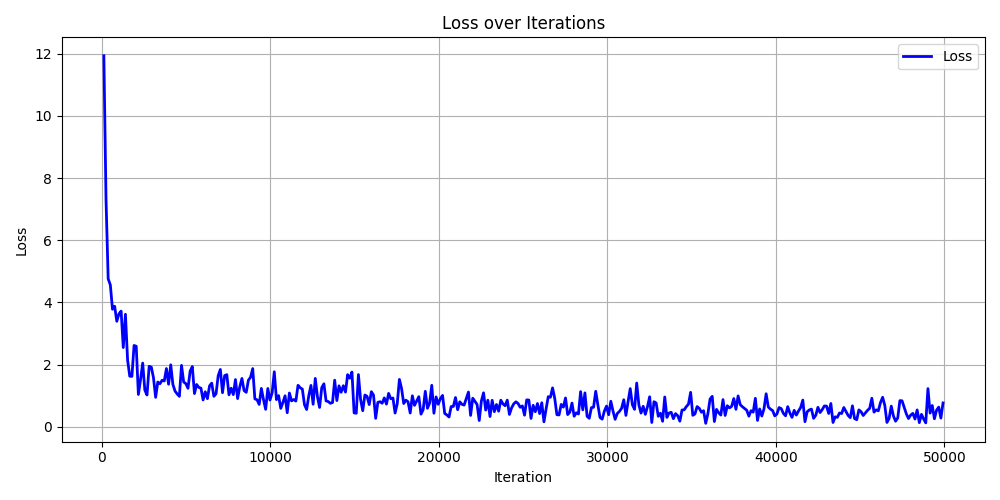
\includegraphics[width=0.95\textwidth]{figures/loss_plot_gpu.png}
  \end{center}
  \caption{A plot of the training loss of a neural network built using MiniTorch on the MNIST dataset.}\label{fig:loss-plot}
\end{figure}


